\subsection{Protocol decision example}\label{sc:protocolDecisionExample}
Figure \ref{recievedSignal_baseStation_air} shows the base station's RF input power of a run around the track from start to finish and figure \ref{recievedSignal_baseStation_air2} shows it for 47 rounds, which equals a marathon, and each round has different fading. Figure \ref{fig:recievedSignal_inRange_halfTrack} shows the in-range of the base station packets which needs to be relayed or not.

%Figure 10
\begin{figure}[h]
	\centering
	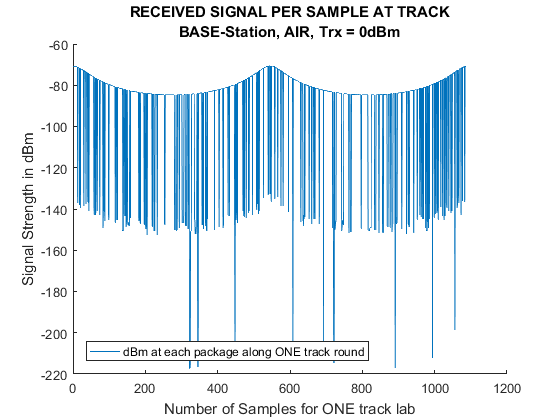
\includegraphics[width=\linewidth]{theory/protocolDecisionExample/fig/recievedSignal_baseStation_air.png}
	\caption{dBm plot of a single run around the track.}
	\label{fig:recievedSignal_baseStation_air}
\end{figure}

\begin{figure}[h]
	\centering
	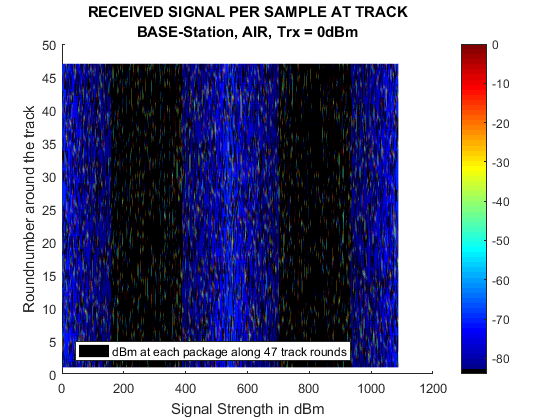
\includegraphics[width=\linewidth]{theory/protocolDecisionExample/fig/recievedSignal_baseStation_air2.png}
	\caption{dBm plot of 47 runs (marathon) around the track.}
	\label{fig:recievedSignal_baseStation_air2}
\end{figure}

%Figure 11
\begin{figure}[h]
	\centering
	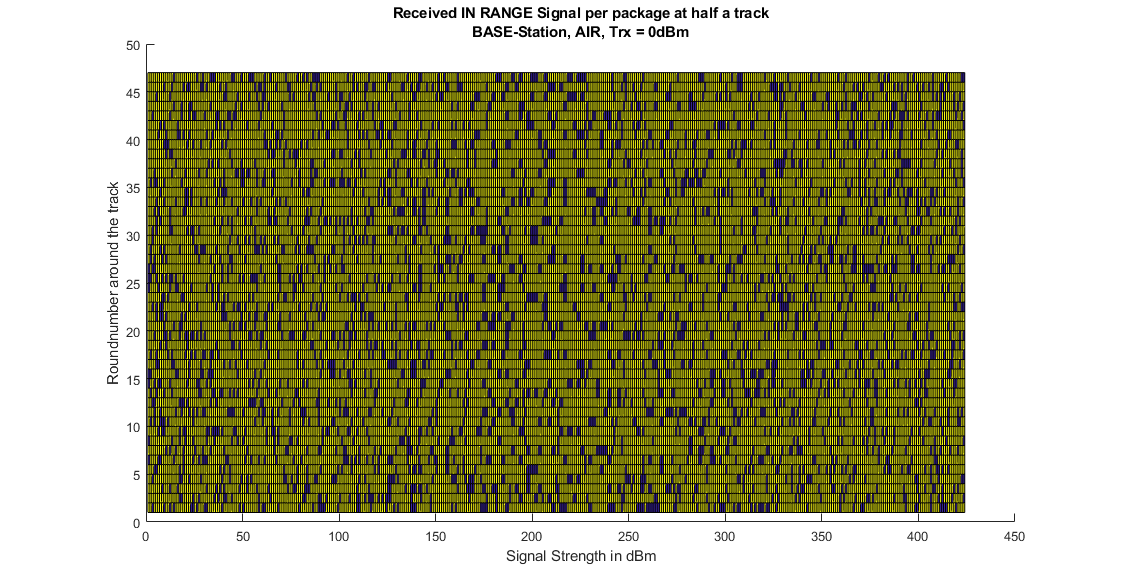
\includegraphics[width=\linewidth]{theory/protocolDecisionExample/fig/recievedSignal_inRange_halfTrack.png}
	\caption{In, half a track, base station RF input power transmitting range ToHopOrNot plot. Blue is relayed packages while yellow is direct package.}
	\label{fig:recievedSignal_inRange_halfTrack}
\end{figure}

\noindent A multi linear regression was fitted on the simulated data with three predictors: Distance, signal strength and whether the packet had been relayed before. The goal was to determine if the node should relay the next packet or not. Since signal strength and distance are strongly correlated in our simulation, due to antenna approximations and the binary behavior of the fading, they cancel each other out, while the previous packet status shows a $10\%$ likelihood of the next packet needing to be relayed. Again, it is expected since the simulations have fading behavior added as a random variable appearing with a $10\%$ likelihood. A real-life trial would be interesting, but is out of scope. Figure \ref{fig:regressionPlot} shows the regression plot with the linear equation added in a legend box.

%Figure 12
\begin{figure}[h]
	\centering
	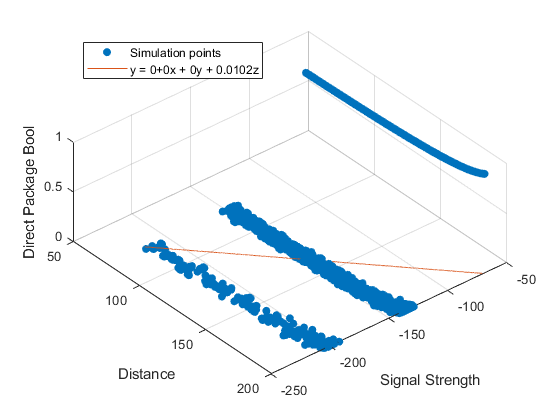
\includegraphics[width=\linewidth]{theory/protocolDecisionExample/fig/regressionPlot.png}
	\caption{Regression plot of the three variables: Distance, signal strength and if previous packet was relayed or not. The regression line is representing a change from direct transmission to relaying.}
	\label{fig:regressionPlot}
\end{figure}